\documentclass[12pt,t,handout]{beamer}
\usepackage{graphicx}
\setbeameroption{show notes}
\setbeamertemplate{note page}[plain]
\usepackage{listings}
\usepackage{datetime}
\usepackage{url}

% specifications for presenter mode
%\beamerdefaultoverlayspecification{<+->}
%\setbeamercovered{transparent}

% math shorthand
\usepackage{amsmath}
\usepackage{amsfonts}
\usepackage{amssymb}
\usepackage{float}
\usepackage{bbm}
\usepackage{bm}
\usepackage{mathtools}
\newcommand{\D}{\mathcal{D}}
\newcommand{\E}{\mathbb{E}}
\newcommand{\F}{\mathcal{F}}
\newcommand{\X}{\mathcal{X}}
\newcommand{\lik}{\mathcal{L}}
\newcommand{\pr}{\mathbb{P}}
\DeclarePairedDelimiterX{\infdivx}[2]{(}{)}{%
  #1\;\delimsize\|\;#2%
}
\newcommand{\infdiv}{D\infdivx}
\DeclarePairedDelimiter{\norm}{\lVert}{\rVert}
\DeclareMathOperator*{\argmin}{arg\,min}
\DeclareMathOperator*{\argmax}{arg\,max}
\newcommand{\openr}{\hbox{${\rm I\kern-.2em R}$}}

% Bibliography
\usepackage{natbib}
\bibpunct{(}{)}{,}{a}{}{;}
\usepackage{bibentry}
\nobibliography*

\def\notescolors{1}
% header.tex: boring LaTeX/Beamer details + macros

% get rid of junk
\usetheme{default}
\beamertemplatenavigationsymbolsempty
\hypersetup{pdfpagemode=UseNone} % don't show bookmarks on initial view


% font
\usepackage{fontspec}
\setsansfont
  [ ExternalLocation = fonts/ ,
    UprightFont = *-regular ,
    BoldFont = *-bold ,
    ItalicFont = *-italic ,
    BoldItalicFont = *-bolditalic ]{texgyreheros}
\setbeamerfont{note page}{family*=pplx,size=\footnotesize} % Palatino for notes
% "TeX Gyre Heros can be used as a replacement for Helvetica"
% I've placed them in fonts/; alternatively you can install them
% permanently on your system as follows:
%     Download http://www.gust.org.pl/projects/e-foundry/tex-gyre/heros/qhv2.004otf.zip
%     In Unix, unzip it into ~/.fonts
%     In Mac, unzip it, double-click the .otf files, and install using "FontBook"

% named colors
\definecolor{offwhite}{RGB}{255,250,240}
\definecolor{gray}{RGB}{155,155,155}

\ifx\notescolors\undefined % slides
  \definecolor{foreground}{RGB}{255,255,255}
  \definecolor{background}{RGB}{24,24,24}
  \definecolor{title}{RGB}{107,174,214}
  \definecolor{subtitle}{RGB}{102,255,204}
  \definecolor{hilit}{RGB}{102,255,204}
  \definecolor{vhilit}{RGB}{255,111,207}
  \definecolor{lolit}{RGB}{155,155,155}
\else % notes
  \definecolor{background}{RGB}{255,255,255}
  \definecolor{foreground}{RGB}{24,24,24}
  \definecolor{title}{RGB}{27,94,134}
  \definecolor{subtitle}{RGB}{22,175,124}
  \definecolor{hilit}{RGB}{122,0,128}
  \definecolor{vhilit}{RGB}{255,0,128}
  \definecolor{lolit}{RGB}{95,95,95}
\fi
\definecolor{nhilit}{RGB}{128,0,128}  % hilit color in notes
\definecolor{nvhilit}{RGB}{255,0,128} % vhilit for notes

\newcommand{\hilit}{\color{hilit}}
\newcommand{\vhilit}{\color{vhilit}}
\newcommand{\nhilit}{\color{nhilit}}
\newcommand{\nvhilit}{\color{nvhilit}}
\newcommand{\lolit}{\color{lolit}}

% use those colors
\setbeamercolor{titlelike}{fg=title}
\setbeamercolor{subtitle}{fg=subtitle}
\setbeamercolor{institute}{fg=lolit}
\setbeamercolor{normal text}{fg=foreground,bg=background}
\setbeamercolor{item}{fg=foreground} % color of bullets
\setbeamercolor{subitem}{fg=lolit}
\setbeamercolor{itemize/enumerate subbody}{fg=lolit}
\setbeamertemplate{itemize subitem}{{\textendash}}
\setbeamerfont{itemize/enumerate subbody}{size=\footnotesize}
\setbeamerfont{itemize/enumerate subitem}{size=\footnotesize}

% page number
\setbeamertemplate{footline}{%
    \raisebox{5pt}{\makebox[\paperwidth]{\hfill\makebox[20pt]{\lolit
          \scriptsize\insertframenumber}}}\hspace*{5pt}}

% add a bit of space at the top of the notes page
\addtobeamertemplate{note page}{\setlength{\parskip}{12pt}}

% default link color
\hypersetup{colorlinks, urlcolor={hilit}}

\ifx\notescolors\undefined % slides
  % set up listing environment
  \lstset{language=bash,
          basicstyle=\ttfamily\scriptsize,
          frame=single,
          commentstyle=,
          backgroundcolor=\color{darkgray},
          showspaces=false,
          showstringspaces=false
          }
\else % notes
  \lstset{language=bash,
          basicstyle=\ttfamily\scriptsize,
          frame=single,
          commentstyle=,
          backgroundcolor=\color{offwhite},
          showspaces=false,
          showstringspaces=false
          }
\fi

% a few macros
\newcommand{\bi}{\begin{itemize}}
\newcommand{\bbi}{\vspace{24pt} \begin{itemize} \itemsep8pt}
\newcommand{\ei}{\end{itemize}}
\newcommand{\ig}{\includegraphics}
\newcommand{\subt}[1]{{\footnotesize \color{subtitle} {#1}}}
\newcommand{\ttsm}{\tt \small}
\newcommand{\ttfn}{\tt \footnotesize}
\newcommand{\figh}[2]{\centerline{\includegraphics[height=#2\textheight]{#1}}}
\newcommand{\figw}[2]{\centerline{\includegraphics[width=#2\textwidth]{#1}}}


%%%%%%%%%%%%%%%%%%%%%%%%%%%%%%%%%%%%%%%%%%%%%%%%%%%%%%%%%%%%%%%%%%%%%%
% end of header
%%%%%%%%%%%%%%%%%%%%%%%%%%%%%%%%%%%%%%%%%%%%%%%%%%%%%%%%%%%%%%%%%%%%%%

% title info
\title{\small Fair Inference Through Semiparametric-Efficient Estimation Over
  Constraint-Specific Paths}
\subtitle{\scriptsize for \textit{New Developments in Nonparametric and
    Semiparametric Statistics},\\
    Joint Statistical Meetings; Vancouver, BC, Canada; 02 Aug.~2018\\[-10pt]}
\author{\href{https://nimahejazi.org}{Nima Hejazi}
       \\[-10pt]
       }
\institute{Group in Biostatistics, and\\
           Center for Computational Biology, \\
           University of California, Berkeley
           \\[4pt]
           
\includegraphics[height=20mm]{Figs/seal-berkeley.png}
           \\[-12pt]
          }
\date{
  \href{https://nimahejazi.org}
      {\tt \scriptsize \color{foreground} nimahejazi.org}
  \\[-4pt]
  \href{https://twitter.com/nshejazi}
      {\tt \scriptsize \color{foreground} Twitter: nshejazi}
  \\[-4pt]
  \href{https://github.com/nhejazi}
      {\tt \scriptsize \color{foreground} GitHub: nhejazi}
}

%%%%%%%%%%%%%%%%%%%%%%%%%%%%%%%%%%%%%%%%%%%%%%%%%%%%%%%%%%%%%%%%%%%%%%%%%%%%%%%%

\begin{document}

% title slide
{
\setbeamertemplate{footline}{} % no page number here
\frame{
  \titlepage

  \vspace{-1em}

  \centerline{\href{http://bit.ly/jsm_fairtmle_2018}{\tt \scriptsize
      \underline{slides}: bit.ly/jsm\_fairtmle\_2018}}
  \vspace{-1.5em}
  \vfill \hfill 
\includegraphics[height=6mm]{Figs/cc-zero.png} \vspace*{-0.5cm}

  \note{This slide deck is for a short presentation on new work in Targeted
    Learning, discussing both the construction of constrained ensemble machine
    learning for the construction of ``fair'' estimates and a novel algorithm
    for computing TML estimators with respect to some contraint functional.

    Slides: {\tt bit.ly/jsm\_fairtmle\_2018}
}
}
}

%%%%%%%%%%%%%%%%%%%%%%%%%%%%%%%%%%%%%%%%%%%%%%%%%%%%%%%%%%%%%%%%%%%%%%%%%%%%%%%%

\begin{frame}[c]{Preview: Summary}
\only<1>{\addtocounter{framenumber}{-1}}

\begin{center}
\begin{itemize}
  \itemsep12pt
  \item Recent work suggests that the widespread use of machine learning
    algorithms has had negative social and policy consequences.
  \item The construction of ``fair'' machine learning algorithms is an active
    area of diverse research.
  \item We propose a general algorithm for constructing ``fair'' optimal
    ensemble machine learning estimators via cross-validation.
  \item We extend Targeted Learning provides a framework for estimating complex
    parameters in nonparametric (infinite-dimensional) statistical models.
  \item Constraints may be imposed as functionals defined over the target
    parameter of interest.
  \item Estimating constrained parameters may be seen as iteratively minimizing
    a loss function along a \textit{constrained} path in the parameter space
    $\Psi$.
\end{itemize}
\end{center}

\note{We'll go over this summary again at the end of the talk. Hopefully, it
  will all make more sense then.
}

\end{frame}

%%%%%%%%%%%%%%%%%%%%%%%%%%%%%%%%%%%%%%%%%%%%%%%%%%%%%%%%%%%%%%%%%%%%%%%%%%%%%%%%

\begin{frame}[fragile,c]{What's fair if machines aren't?}

\begin{center}
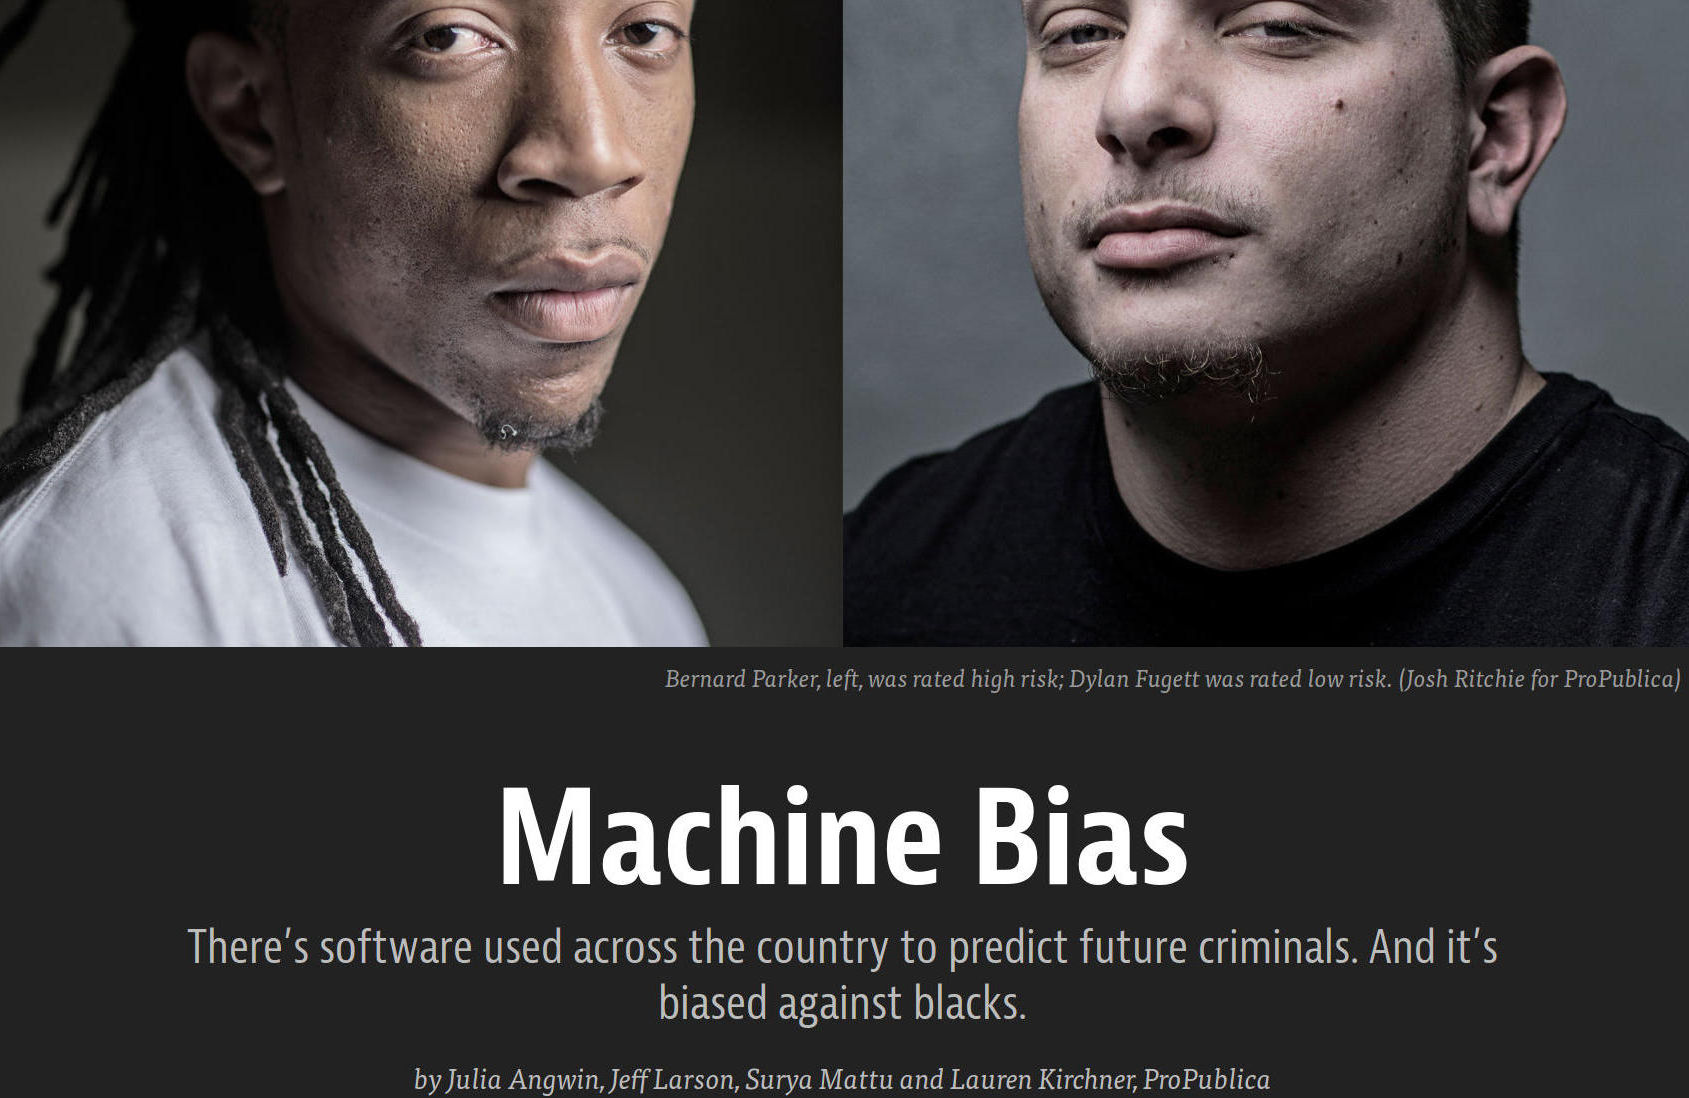
\includegraphics[height=70mm]{Figs/propublica.jpg}
\end{center}

\note{
}

\end{frame}

%%%%%%%%%%%%%%%%%%%%%%%%%%%%%%%%%%%%%%%%%%%%%%%%%%%%%%%%%%%%%%%%%%%%%%%%%%%%%%%%

\begin{frame}[fragile,c]{Fairness is machine learning?}

\begin{center}
\begin{minipage}[c]{11.25cm}
\begin{semiverbatim}
\lstset{basicstyle=\normalsize}
\begin{lstlisting}[linewidth=11.25cm]
  Another potential result: a more diverse
  workplace. The software relies on data
  to surface candidates from a wide variety
  of places...free of human biases. But
  software is not free of human influence.
  Algorithms are written and maintained by
  people...As a result...algorithms can
  reinforce human prejudices.

  -Miller (2015)
\end{lstlisting}
\end{semiverbatim}
\end{minipage}
\end{center}

\note{Obviously, it's important to explain the motivating example here.}

\end{frame}

%%%%%%%%%%%%%%%%%%%%%%%%%%%%%%%%%%%%%%%%%%%%%%%%%%%%%%%%%%%%%%%%%%%%%%%%%%%%%%%%

\begin{frame}[c]{Addressing bias in a technical manner}

\begin{center}
\begin{itemize}
  \itemsep12pt
  \item The careless use of machine learning may induce \textit{unjustified}
    bias.
  \item Problematic discrimination by ML approaches leads to solutions with
    \textit{practical irrelevance}.
  \item Ill-considered discrimination by ML approaches leads to solutions that
    are \textit{morally problematic}.
  \item Two doctrines of discrimination:
    \begin{enumerate}
      \item Disparate treatment: formal or intentional
      \item Disparate impact: unjustified or avoidable
    \end{enumerate}
\end{itemize}
\end{center}

\note{
  Considering and treating bias using a technical approach is an important way
  of dealing with the potential negative consequences of machine learning.
}

\end{frame}

%%%%%%%%%%%%%%%%%%%%%%%%%%%%%%%%%%%%%%%%%%%%%%%%%%%%%%%%%%%%%%%%%%%%%%%%%%%%%%%%

\begin{frame}[c]{Background, data, notation}

\begin{center}
\begin{itemize}
  \itemsep12pt
  \item An observational unit: $O = (W, X, Y)$, where $W$ is baseline
    covariates, $X$ a sensitive characteristic, $Y$ an outcome of interest.
  \item Consider $n$ i.i.d.~copies $O_1, \ldots, O_n$ of $O \sim P_0 \in
    \mathcal{M}$.
  \item Here, $\mathcal{M}$ is an infinite-dimensional statistical model (i.e.,
    indexed by an infinite-dimensional vector).
  \item We discuss the estimation of a target parameter $\psi : \mathcal{M}
    \rightarrow \mathbb{R}$, where
    $$\Psi(P_0) = \argmin_{\psi \in \Psi} \E_{P_0}L(\psi)$$
\end{itemize}
\end{center}

\note{
  We just need to see this to get a feel for what's going to be happening with
  the derivation of constraint-specific paths.
}

\end{frame}

%%%%%%%%%%%%%%%%%%%%%%%%%%%%%%%%%%%%%%%%%%%%%%%%%%%%%%%%%%%%%%%%%%%%%%%%%%%%%%%%

\begin{frame}[c]{Just a few fairness criteria}

\begin{center}
\begin{itemize}
  \itemsep8pt
  \item Let $C: (X, W) \to Y \in \{0, 1\}$ be a classifier; $X \in \{a, b\}$.
  \item Demographic parity: $\pr_{(X = a)}(C = 1) = \pr_{(X = b)}(C = 1)$
  \item Accuracy parity: $\pr_{(X = a)}(C = Y) = \pr_{(X = b)}(C = Y)$
  \item True positive parity: $\pr_{(X = a)}(C = 1 \mid Y = 1) =
    \pr_{(X = b)}(C = 1 \mid Y = 1)$
  \item False positive parity: $\pr_{(X = a)}(C = 1 \mid Y = 0) =
    \pr_{(X = b)}(C = 1 \mid Y = 0)$
  \item Positive predictive value parity: $\pr_{(X = a)}(Y = 1 \mid C = 1) =
    \pr_{(X = b)}(Y = 1 \mid C = 1)$
  \item Negative predictive value parity: $\pr_{(X = a)}(Y = 1 \mid C = 0) =
    \pr_{(X = b)}(Y = 1 \mid C = 0)$
\end{itemize}
\end{center}

\note{
  It's a jungle out there
}

\end{frame}

%%%%%%%%%%%%%%%%%%%%%%%%%%%%%%%%%%%%%%%%%%%%%%%%%%%%%%%%%%%%%%%%%%%%%%%%%%%%%%%%

\begin{frame}[c]{Wait, where did the fairness go?}

\begin{center}
\begin{itemize}
  \itemsep12pt
  \item Goal: estimate $\Psi(P_0) = \E_{P_0}(Y \mid X, W)$.
  \item Let $Y \in \{0, 1\}$ and use negative log-likelihood loss:
    $$L(\psi) = -(Y \log(\pr(Y \mid X, W)) + (1 - Y) \log(1 -
    \pr(Y \mid X, W)))$$
  \item Fairness criterion --- \textit{equalized odds}:
    $$\begin{aligned}
      \Theta_{\psi}(P_0) = \sum_y \{&\E_{P_0}(L(\psi)(O) \mid X = 1, Y = y) \\ -
      &\E_{P_0}(L(\psi)(O) \mid X = 0, Y = y)\}^2
    \end{aligned}$$
  \item Let $\Theta_{\psi}(P_0): \mathcal{M} \rightarrow \openr$ be a pathwise
    differentiable \textit{functional} for each $\psi \in \Psi$.
\end{itemize}
\end{center}

\note{
  Equalized odds simultaneously enforces both true positive parity and false
  positive parity.
}

\end{frame}

%%%%%%%%%%%%%%%%%%%%%%%%%%%%%%%%%%%%%%%%%%%%%%%%%%%%%%%%%%%%%%%%%%%%%%%%%%%%%%%%

\begin{frame}[c]{Constrained functional parameters}

\begin{center}
\begin{itemize}
  \itemsep12pt
  \item Estimate target parameter under a constraint:
    $$\Psi(P) = \argmin_{\psi \in \Psi, \Theta_{\psi}(P) = 0} \E_PL(\psi)$$
  \item Goal: estimate $\Psi^*(P)$, the projection of $\Psi(P)$ onto the
    subspace $\Psi^*(P) = \{\psi \in \Psi: \Theta_{\psi}(P) = 0\}$:
    $$(\Psi^*, \lambda) = (\Psi^*(P), \Lambda(P)) \equiv \argmin_{\psi \in \Psi,
      \lambda} \E_PL(\psi) + \lambda \Theta_{\psi}(P).$$
  \item \textit{Lemma}: If $\widetilde{\Psi}(P) = (\Psi^*(P), \Lambda(P))$ is
    the minimizer of the Lagrange multiplier penalized loss, then
    $$\Psi^*(P) = \argmin_{\psi \in {\bf \Psi}, \Theta_{\psi}(P) = 0}
      \E_{P}L(\psi).$$
\end{itemize}
\end{center}

\note{
}

\end{frame}

%%%%%%%%%%%%%%%%%%%%%%%%%%%%%%%%%%%%%%%%%%%%%%%%%%%%%%%%%%%%%%%%%%%%%%%%%%%%%%%%

\begin{frame}[c]{Learning with constrained parameters}

\begin{center}
\begin{itemize}
  \itemsep14pt
  \item Risk function: $R(\widetilde{\psi} \mid P) \equiv P_nL(\psi^*) +
    \lambda \Theta(\psi^* \mid P)$, where $\widetilde{\psi} = (\psi^*,
    \lambda)$
  \item For $\widetilde{\psi}(P_n) = (\hat{\Psi}^*(P_n), \hat{\lambda}(P_n))$ of
    $\widetilde{\Psi}(P_0)$, and sample splitting scheme $B_n \in \{0, 1\}^n$:
    $$R_0(\widetilde{\psi}, P_n) = \E_{B_n} P_0L(\hat{\Psi}^*(P_{n, B_n}^0)) +
      \hat{\Lambda}(P_n) \E_{B_n} \Theta(\hat{\Psi}^*(P_{n, B_n}^0) \mid P_0)$$
\end{itemize}
\end{center}

\note{
  \begin{itemize}
    \item Here $P_{n, B_n}^0$ denotes the empirical distribution of the training
      sample.
  \end{itemize}
}

\end{frame}

%%%%%%%%%%%%%%%%%%%%%%%%%%%%%%%%%%%%%%%%%%%%%%%%%%%%%%%%%%%%%%%%%%%%%%%%%%%%%%%%

\begin{frame}[c]{Learning with constrained parameters}

\begin{center}
\begin{itemize}
  \itemsep14pt
  \item Cross-validated risk:
    \begin{align}
      R_{n, CV}(\tilde{\psi}, P_n) =& E_{B_n}P_{n, B_n}^1L(\hat{\Psi}^*(P_{n,
        B_n}^0)) \\ &+ \hat{\Lambda}(P_n) E_{B_n} \Theta(\hat{\Psi}^*(P_{n,
        B_n}^0) \mid P_{n, B_n}^*)
    \end{align}
  \item Given candidate estimators $\widetilde{\psi}_j(P_n) =
    (\hat{\Psi}_j^*(P_n), \hat{\Lambda}_j(P_n))$, $j = 1, \ldots, J$, the CV
    selector is given by: $J_n = \argmin_j R_{n, CV}(\widetilde{\psi}_j, P_n)$.
  \item We may define an optimal estimate of $\widetilde{\Psi}$ by
    $\widetilde{\psi}_n \equiv \widetilde{\psi}_{J_n}(P_n) =
    (\hat{\Psi}_{J_n}(P_n), \hat{\lambda}_{J_n}(P_n))$
\end{itemize}
\end{center}

\note{
}

\end{frame}

%%%%%%%%%%%%%%%%%%%%%%%%%%%%%%%%%%%%%%%%%%%%%%%%%%%%%%%%%%%%%%%%%%%%%%%%%%%%%%%%

\begin{frame}[c]{Mappings with constrained learners}

\begin{center}
A straightforward approach to generating estimators of the constrained parameter
would be to simply generate a mapping according to the following simple process:

\vspace*{1em}

\begin{enumerate}
  \itemsep12pt
  \item Generate an unconstrained estimate $\psi_n$ of the unconstrained
    parameter $\psi_0$,
  \item Map an estimator $\Theta_{\psi_n, n}$ of the constraint
    $\Theta_{\psi_n}(P_0)$ into the path $\psi_{n, \lambda}$. The corresponding
    solution $\psi_n^* = \psi_{n, \lambda_n}$ of $\Theta_{\psi_{n, \lambda_n},
      n} = 0$ generates an estimator of the constrained parameter.
\end{enumerate}
\end{center}

\note{
}

\end{frame}

%%%%%%%%%%%%%%%%%%%%%%%%%%%%%%%%%%%%%%%%%%%%%%%%%%%%%%%%%%%%%%%%%%%%%%%%%%%%%%%%

\begin{frame}[c]{Constraint-specific paths}

\begin{center}
\begin{itemize}
  \item Consider $\psi_{0, \lambda} = \argmax_{\psi \in \Psi} \E_{P_0}L(\psi) +
    \lambda \Theta_0(\psi)$.
  \item $\{\psi_{0, \lambda} : \lambda\}$ represents a path in the parameter
    space $\Psi$ through $\psi_0$ at $\lambda = 0$.
  \item This is a \textit{constraint-specific path}, as it produces an estimate
    under the desired functional constraint.
  \item Leverage this construction to map an initial estimator of the
    unconstrained parameter $\psi_0$ into its corresponding constrained version
    $\psi_0^*$.
\end{itemize}
\end{center}

\note{
}

\end{frame}

%%%%%%%%%%%%%%%%%%%%%%%%%%%%%%%%%%%%%%%%%%%%%%%%%%%%%%%%%%%%%%%%%%%%%%%%%%%%%%%%

\begin{frame}[c]{Future work}

\begin{center}
\begin{itemize}
  \itemsep12pt
  \item Further generalization of constraint-specific paths: the solution path
    $\{\psi_{0, \lambda}: \lambda\}$ in the parameter space $\Psi$ through
    $\psi_0$ at $\lambda = 0$.
  \item Further develop relation between constraint-specific paths and universal
    least favorable submodels (Efron's least favorable families).
  \item Integration of the approach of constraint-specific paths with classical
    classical targeted maximum likelihood estimation --- in particular, what, if
    any, are the implications for inference?
  \item Try our approach out with practical constraint-type problems (e.g.,
    fairness via equalized odds, physician knowledge in prediction).
\end{itemize}
\end{center}

\note{
}

\end{frame}

%%%%%%%%%%%%%%%%%%%%%%%%%%%%%%%%%%%%%%%%%%%%%%%%%%%%%%%%%%%%%%%%%%%%%%%%%%%%%%%%

\begin{frame}[c]{Review: Summary}

\begin{center}
\begin{itemize}
  \itemsep12pt
  \item Targeted Learning provides a framework for estimating complex parameters
    in nonparametric (infinite-dimensional) statistical models.
  \item Constraints may be imposed as functionals defined over the target
    parameter of interest.
  \item Estimating constrained parameters may be seen as iteratively minimizing
    a loss function along a \textit{constrained} path in the parameter space
    $\Psi$.
  \item Optimal nonparametric estimates of parameters (and constituent parts
    thereof) may be obtained with Super Learning (i.e., stacked regression,
    ensemble models).
\end{itemize}
\end{center}

\note{It's always good to include a summary.}

\end{frame}

%%%%%%%%%%%%%%%%%%%%%%%%%%%%%%%%%%%%%%%%%%%%%%%%%%%%%%%%%%%%%%%%%%%%%%%%%%%%%%%%

% don't want dimming with references
%\setbeamercovered{}
%\beamerdefaultoverlayspecification{}

\begin{frame}[c,allowframebreaks]{References}

\bibliographystyle{apalike}
\nocite{*}
\bibliography{references}

%\note{Here's some work we've talked about. Go check these out if interested.}

\end{frame}

%%%%%%%%%%%%%%%%%%%%%%%%%%%%%%%%%%%%%%%%%%%%%%%%%%%%%%%%%%%%%%%%%%%%%%%%%%%%%%%%

\begin{frame}{Acknowledgments}

\vspace{18pt}

\begin{tabular}{@{}l@{\hspace{1.5cm}}l@{}}
Mark J.~van der Laan & \footnotesize \lolit University of California, Berkeley
\end{tabular}

\vspace{10mm}

\underline{Funding source}:\\
National Library of Medicine (of NIH): T32-LM012417--02

\note{
}

\end{frame}

%%%%%%%%%%%%%%%%%%%%%%%%%%%%%%%%%%%%%%%%%%%%%%%%%%%%%%%%%%%%%%%%%%%%%%%%%%%%%%%%

\begin{frame}[c]{Thank you.}

\Large
Slides: \href{https://bit.ly/jsm_fairtmle_2018}{bit.ly/jsm\_fairtmle\_2018}
\quad 
\includegraphics[height=5mm]{Figs/cc-zero.png}

\vspace{2mm}
\href{http://nimahejazi.org}{\tt nimahejazi.org}

\vspace{2mm}
\href{https://twitter.com/nshejazi}{\tt Twitter: nshejazi}

\vspace{2mm}
\href{https://github.com/nhejazi}{\tt GitHub: nhejazi}

\note{Here's where you can find me, as well as the slides for this talk.}

\end{frame}

%%%%%%%%%%%%%%%%%%%%%%%%%%%%%%%%%%%%%%%%%%%%%%%%%%%%%%%%%%%%%%%%%%%%%%%%%%%%%%%%

\end{document}

